\documentclass[11pt,a4paper]{article}
\usepackage{amsmath,amssymb}
\usepackage{graphicx}
\usepackage{booktabs}
\usepackage{float}
\usepackage{geometry}
\geometry{margin=0.9in}
\usepackage{xcolor}
\usepackage{hyperref}
\hypersetup{colorlinks=true, urlcolor=cyan, linkcolor=blue}
\setlength{\parskip}{4pt}\setlength{\parindent}{0pt}

\title{\textbf{Aims 1 and 2: Findings Brief} \\ \large Measuring the multilinguality of
LLMs: ten findings \\ \normalsize (methods, statistics, and the error ledger are in the
accompanying technical report)}
\author{Waiz Khan \\ \texttt{wkhan12@jh.edu}}
\date{July 2026}

\begin{document}
\maketitle

\textbf{The assignment} (proposal \S3.1.4): build an intrinsic metric of LLM
multilinguality. \textbf{The contribution}: one primary metric, the
\textbf{Language-Factor Share} (LFS); the share of systematic
representation variance attributable to language rather than shared concept
structure, an exact two-way variance decomposition on a balanced translation grid; with a validation methodology (``confounder-adjusted validity'') that removes observable
confounds before any claim is made. Retrieval alignment, tail analysis
(Alignment-at-Risk), downstream performance, and generation-time context use
serve as \emph{validation instruments}, not additional definitions of
multilinguality. \textbf{Scale}: 17 open models (0.6B--9B), 122--128
languages, all claims either pre-registered or confound-controlled.

\section*{Finding 1: Your \S3.1.1 hypothesis, measured}
The proposal asks ``how strong the language component in the representation
is.'' The \textbf{Language-Factor Share} (LFS) is a direct operational
measure of it, per layer:
every model shows language-specific $\to$ shared $\to$ language-specific
processing, and the depth of the shared dip varies almost $10\times$ across
models (0.04--0.34). By construction, LFS measures the \emph{additive,
systematic} language share of representation variance; language-specific
rotations or concept-specific distortions fall outside it. A pre-registered
falsification test suite has since \emph{measured} that boundary: rotation is
0.06--0.2\% of real cross-language misalignment (offset$+$scale:
63--97\%), it does not predict performance beyond observables, and the one
gaming attack that is missed by every alignment metric tested (global collapse; MEXA included) is caught exactly by a validated variance-preservation
check.

\begin{center}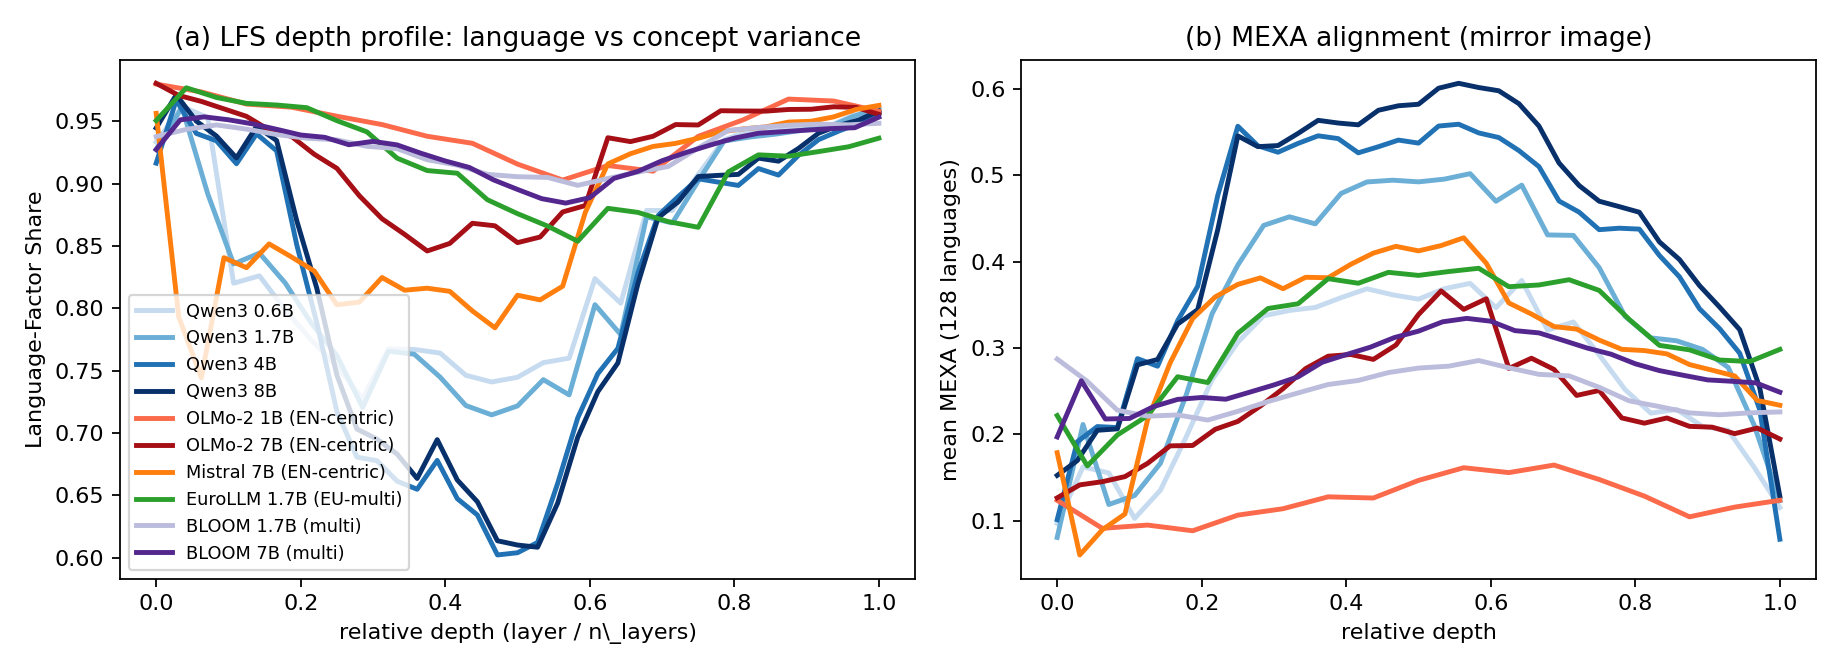
\includegraphics[width=0.95\textwidth]{figs/fig1_lfs_depth_profile.png}\end{center}

\section*{Finding 2: The depth profile has two events, not one}
Pre-registered and confirmed twice: models abandon the input language's
\emph{script} early ($\sim$5--20\% depth) but \emph{meanings} converge only
mid-network ($\sim$30--50\%). Surface form and semantics run on different
schedules.

\begin{center}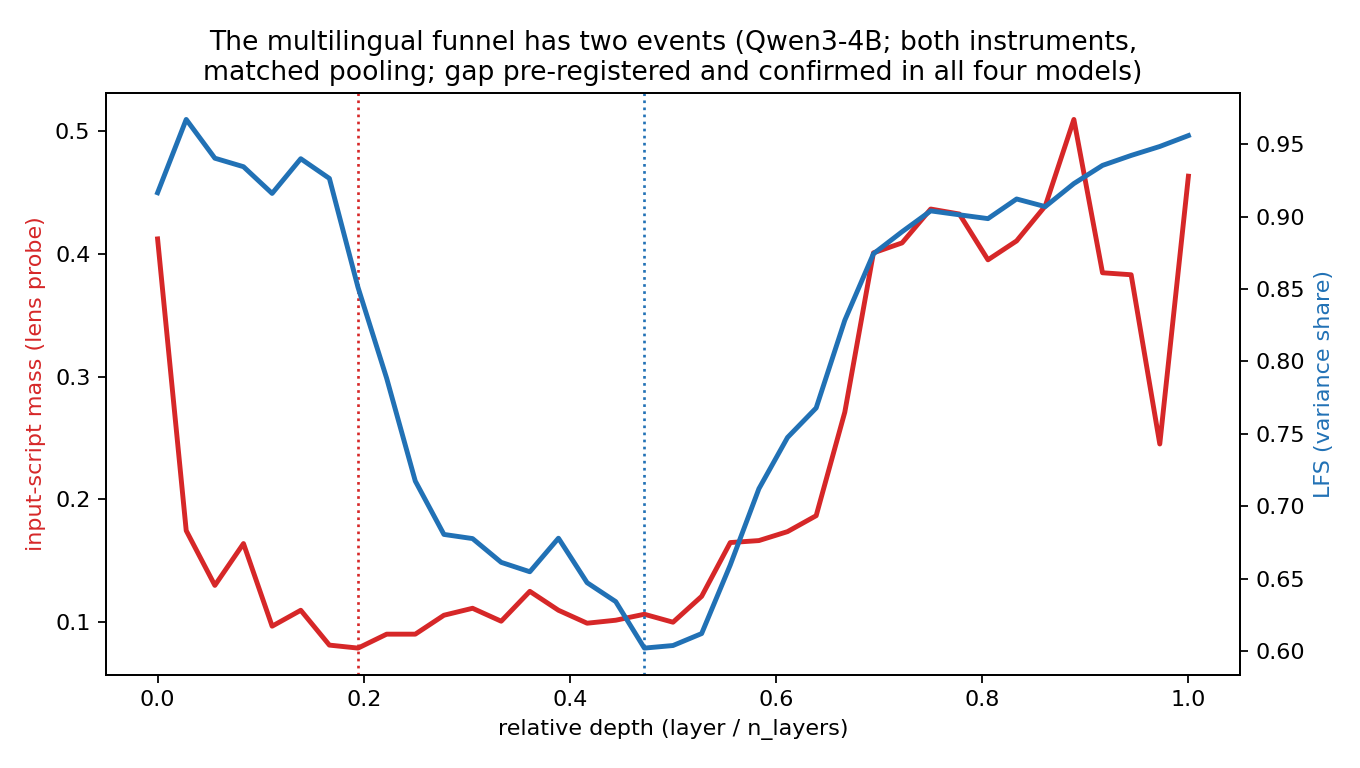
\includegraphics[width=0.72\textwidth]{figs/fig12_twoevents.png}\end{center}

\section*{Finding 3: Family separates more than scale (in this grid)}
Scale deepens the shared space within a family (Qwen3: dip $0.21 \to 0.34$;
low-resource alignment $\times 6$), but between-family differences dwarf the
within-family trend (``family'' bundles data mixture, token budget,
tokenizer, and curriculum; an observational contrast, not a causal
claim): Qwen3-1.7B out-converges every other lab's 7B. \textbf{BLOOM (deliberately
46-language) has the shallowest concept space of all, unchanged from 1.7B
to 7B}: its alignment concentrates at the embedding layer (surface form, not
meaning). \emph{Coverage is a data property; convergence is a training
property.} For Aim~2 this is the license: the quantity is set by training
choices, not an automatic gift of scale.

\section*{Finding 4: ``Thinks in English'' is resource-graded and fading}
A multilingual latent factor predicts each language's representations better
than English does (113 to 124 of 127 languages depending on the model, 124 for most; confound-controlled; a modest
$+0.08\,R^2$ after the smoothness correction). English is the best
single bridge for high-resource targets (9/10) but almost never for
low-resource ones (1/8, where Swahili, Hindi, and Indonesian mediate regionally),
and its hub share \emph{falls} with scale (45$\to$25 of 127 across Qwen3
sizes). Bonus for \S3.1.2: mid-layer states reach max cosine $\sim$0.10 to
\emph{any} output embedding; the Logit Lens is weakest exactly where the
literature applies it.

\section*{Finding 5: The mean hides the tail, and the tail is semantic}
Mid-resource languages pass average-based checks while their worst-decile
sentences sit at retrieval failure. Measure those sentences: named entities
and numerals are alignment \emph{anchors}; what fails is discourse-dependent
meaning (``Interest remained high after the hearing''), culturally-bound
vocabulary, and crowded boilerplate. \textbf{Alignment-at-Risk} (AaR)
reports this tail; means cannot. At the 1,500-sentence scale ($n{=}1500$/language)
this is the \emph{most common} condition, not an anecdote: 40--50\% of languages
in the strongest models are mean-positive but tail-negative (Qwen3-8B:
Turkish and Greek carry means of $+0.13$ over worst-percentile margins of
$-0.26$ and $-0.24$).

\begin{center}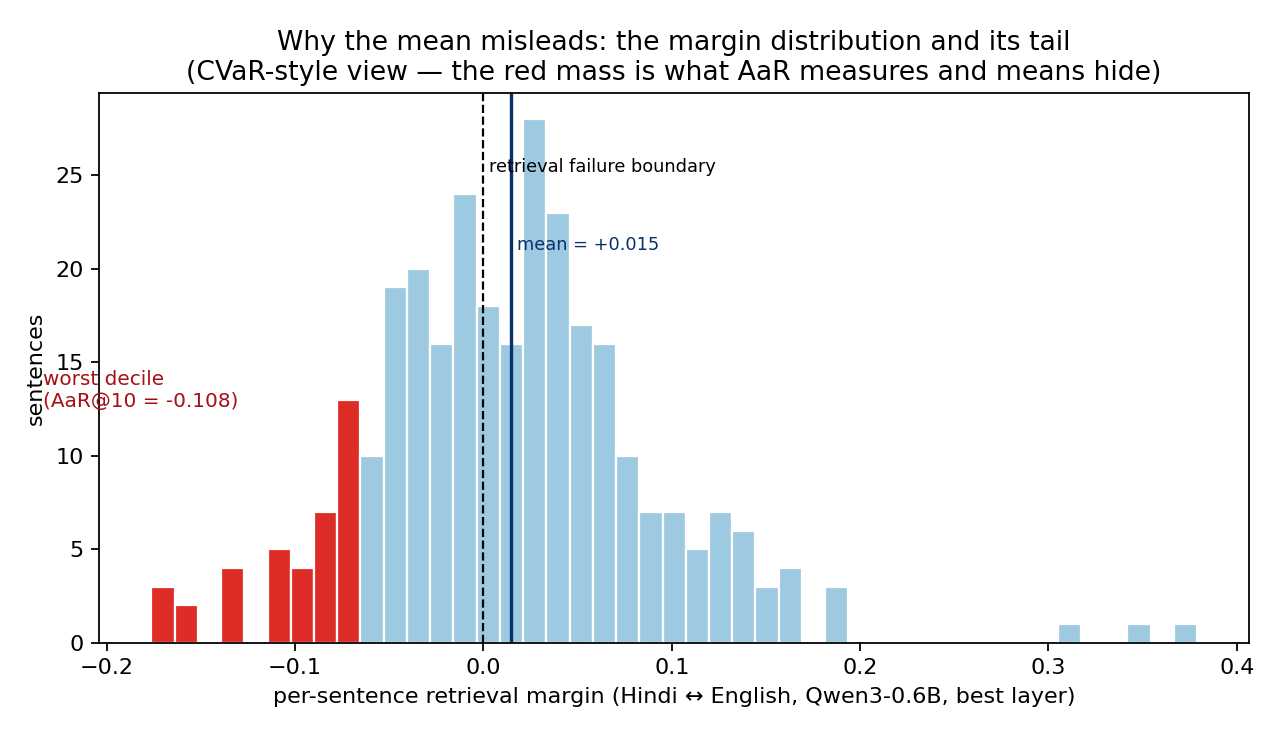
\includegraphics[width=0.8\textwidth]{figs/fig14_cvar.png}\end{center}

\section*{Finding 6: Confounder-adjusted validity: on our grid, the standard
validation number is $\sim$40--60\% confound}
Intrinsic metrics are validated by raw correlation with per-language
performance; but data-rich languages score high on both. Partialling out
data size, family, script, and tokenizer cost: the confounder-adjusted residual range is
$\rho \approx 0.19$--$0.31$ (raw: 0.50--0.53). Real signal survives (the metrics are not merely token-counting), but on this model--language grid and
benchmark, the raw numbers are roughly half confound. (Applied to our own
best number too; see Finding~7.) The July figure of about 0.59 on a benchmark-capable subset is withdrawn: it is not reproducible from any stored artifact, and a re-derivation gives 0.487 [0.365, 0.554].

\begin{center}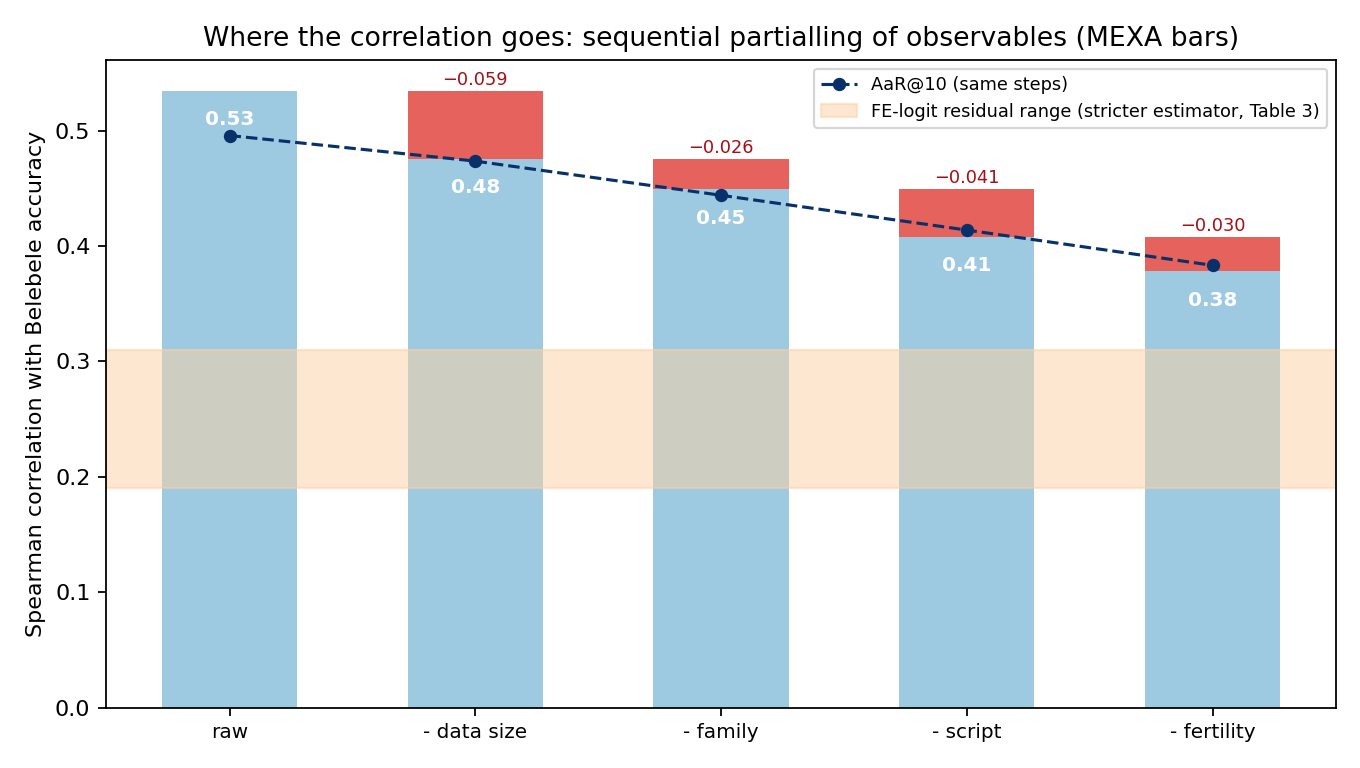
\includegraphics[width=0.72\textwidth]{figs/fig11_waterfall.png}\end{center}

\section*{Finding 7: The shared-space measurements predict behavior
beyond observables}
Pre-registered: per-language alignment, measured at the layer the variance
decomposition identifies, predicts how much a model actually
\emph{uses} a foreign-language context sentence during generation
(mismatched-context controlled, 40 languages). The chain: LFS locates the
shared region; alignment in that region predicts behavior; the structure
LFS finds is behaviorally meaningful. Confounder-adjusted by the same
machinery as Finding~6: pooled residual $\rho = 0.67$
(language-clustered CI $[0.55, 0.77]$; strictest per-language treatment
$\rho = 0.46$, $p = 0.004$).

\textbf{This chain is observational, and it has now been tested under
intervention.} A six-condition training study at three seeds directly optimized
LFS downward by five different objectives. In every condition, at every seed, tail
alignment moved down with it (Pearson $+0.924$ across eighteen condition-seed
points), the opposite of the association seen across pretrained models. The
association therefore does not transfer to these interventions. That is a
limit on \emph{use}, not a refutation of the measurement: LFS is a
measurement and is not a training target.

\begin{center}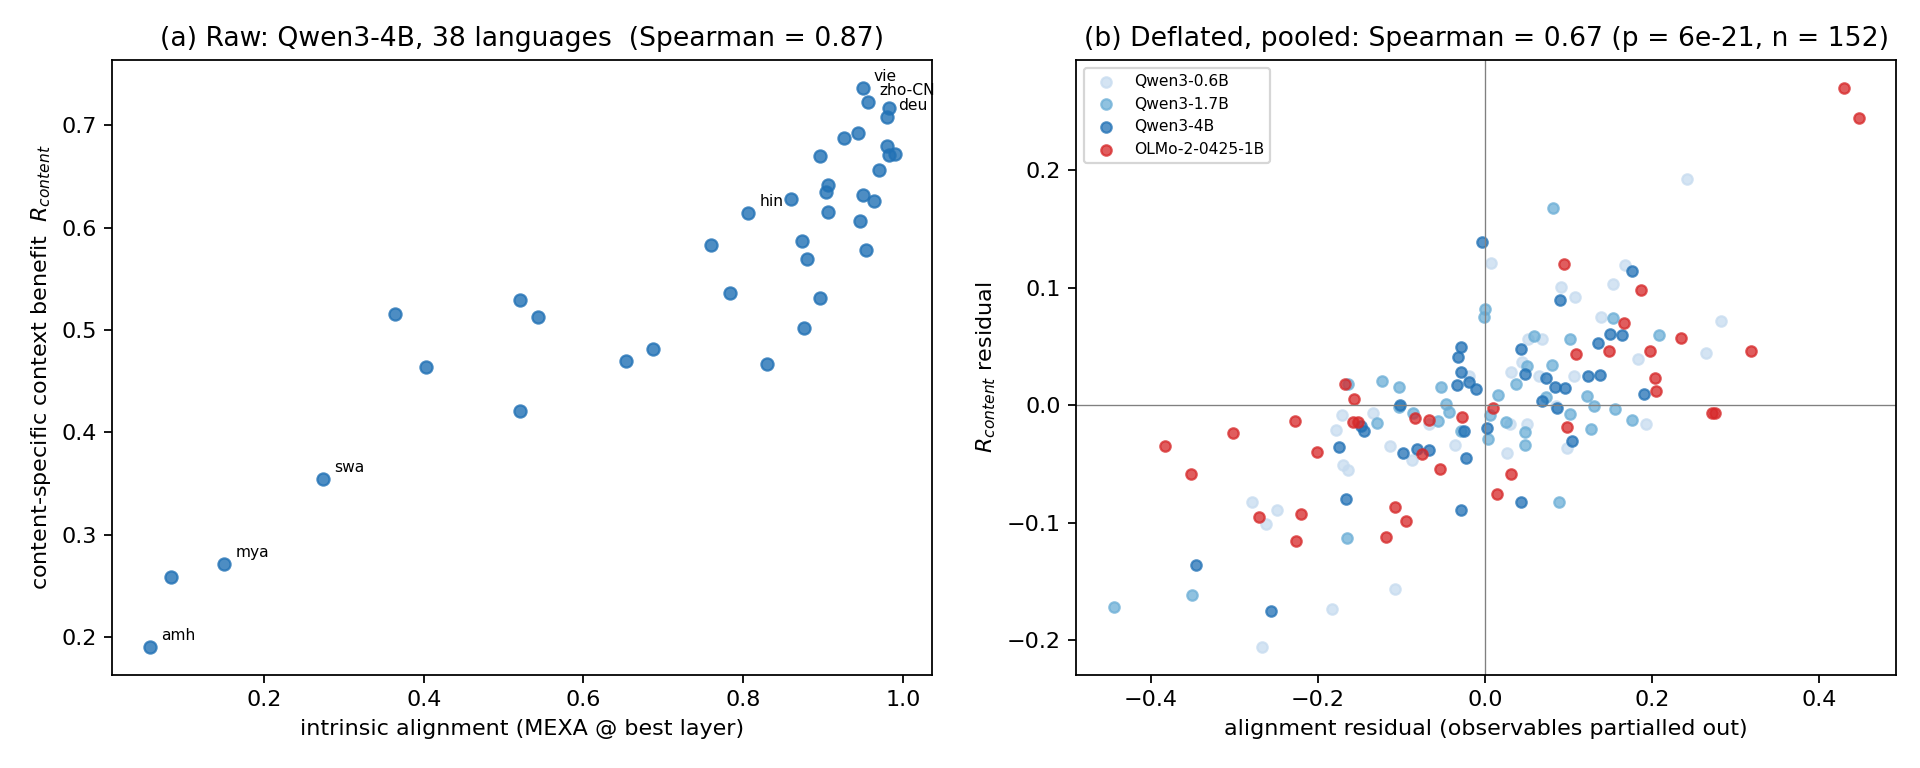
\includegraphics[width=0.95\textwidth]{figs/fig10_b2scatter.png}\end{center}

\section*{Finding 8: Risk-adjusted model comparison}
Mean accuracy and worst-decile accuracy give different answers; the
mean-versus-tail view makes dominance visible immediately, and exposes a hard
floor: $\sim$30 languages have no usable alignment in \emph{any} open model
under 8B; and 28 of 122 Belebele languages are absent from both major
public web-corpus censuses.

\begin{center}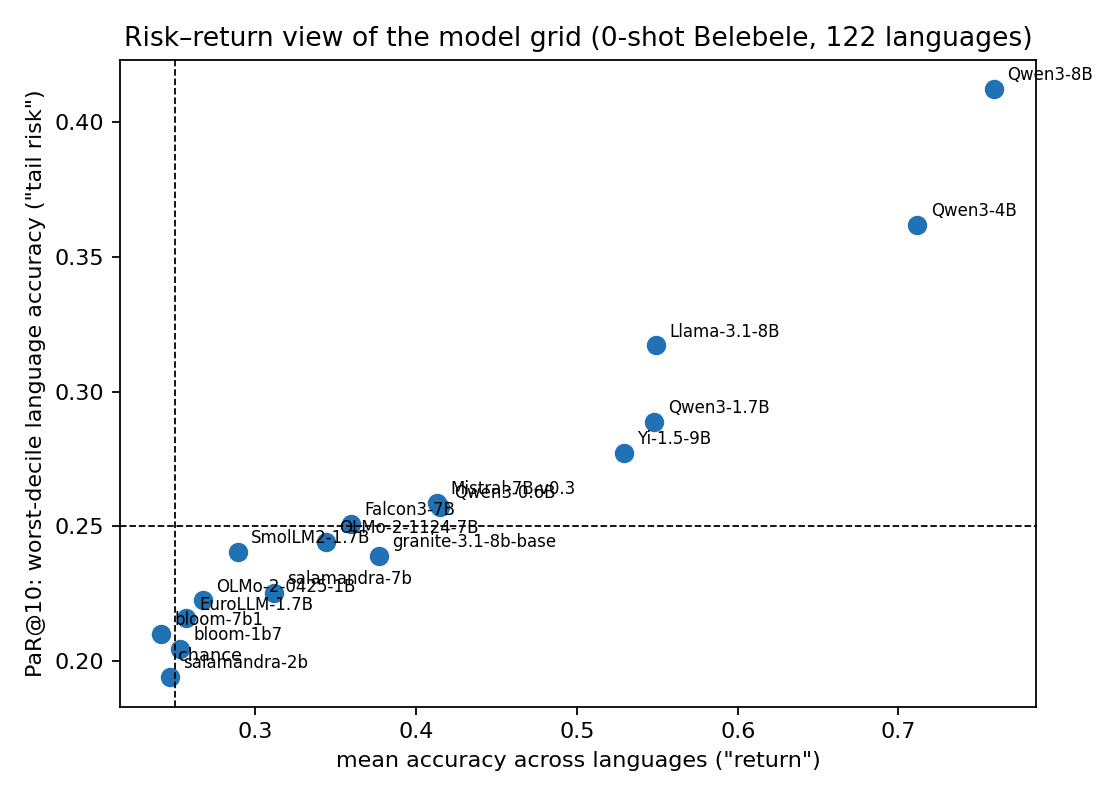
\includegraphics[width=0.6\textwidth]{figs/fig13_riskreturn.png}\end{center}

\section*{Finding 9: The prospective test: four of four, blind}
The suite was designed on 10 models, so two \emph{held-out} families
(SmolLM2, Falcon3) were run through a frozen pre-registered protocol.
\textbf{All four blind predictions passed}: the depth profiles matched their
training-recipe class under blind scoring (SmolLM2 dip 0.068 = the EN-centric
class; Falcon3 0.140 = intermediate); the attribution criterion held; held-out
validity \emph{exceeded} the development-grid confidence interval; and the
preregistered prediction P4, a difference between the tail measure AaR and MEXA on the benchmark-capable subgroup, passed on the one held-out model that qualified ($\Delta = +0.14$, CI $[+0.03, +0.26]$); it is recorded because it was preregistered and is not used as a claim about one measure over another; the retraction was pre-committed had it failed. The metric generalized to both unseen families (one
benchmark-capable).

\section*{Finding 10: the Aim-2 study, and a defect in our own summary
statistic (pre-registered)}
Twenty-eight training conditions across four objective families, three seeds each,
against the proposal's own specifications. \textbf{Every condition fails its frozen
criteria}, and the way they fail is the finding.

The objective \S3.2.2 specifies, a squared difference between matched word
representations, is globally minimized at $h=0$. It degenerated exactly as
pre-registered: representation norms fell \textbf{89\%}. \textbf{Neither our
metric nor the field's standard retrieval metric detected it.} Both are
scale-invariant, and the condition that collapsed its own scale posted the \emph{best}
retrieval and the \emph{best} tail alignment in the study, clearing both
pre-registered thresholds, while the condition that stayed sound gained nothing.

The decomposition underneath LFS separates those two models by a factor of
twenty in raw concept variance. The ratio
$V_{\text{lang}}/(V_{\text{lang}}+V_{\text{concept}})$ divides that difference
out by construction. \textbf{The corrective is to report the component profile
$(V_{\text{lang}}, V_{\text{concept}}, \text{residual}, \lVert h\rVert)$
rather than a single share}; the profile catches every failure in this
study, the share catches none.

Two further results. A concept-variance guard is \emph{necessary and
structurally insufficient}: its hinge is bounded above by 0.81 while the
alignment term starts near 600, so no coefficient restrains it, and a
thousandfold weight sweep saturates. And code-switched data (\S3.2.1) shows no
detectable benefit at any switch rate while costing 17 to 47 points of
perplexity on languages outside the replay mixture.

Aim 1 built the instrument; Aim 2 established what it must not be used for,
and what its summary statistic must not hide.

\vspace{1mm}\hrule\vspace{2mm}
{\small \textbf{How these claims were validated}: every main claim was either
pre-registered before running or adjusted for observables. The
pre-registration ledger totals \textbf{26 predictions, 18 passed}: 13
experimental predictions across two rounds (9 passed; 4 failed, all
productive), 4/4 blind prospective predictions, and a 28-condition Aim-2 study
scored against pre-committed criteria (5 word-level predictions, 4 passed).
\textbf{Ten} self-caught errors are documented
with mechanisms in the full report's ledger. Code, data pipeline, and
protocols are release-ready.}

\end{document}
